
\begin{savequote}[8cm]

  \qauthor{}
\end{savequote}



\chapter{Ethnographic Results\label{chap:ethnoResults}}

\minitoc






                                      \begin{CJK}{UTF8}{gbsn}

%\section{Ethnographic evidence for a relationship between joint action and social bonding}

\section{Introduction}

In this chapter I consider ethnographic evidence that bears upon the research hypotheses set out in this dissertation concerning a general account of team click.  In particular, I ask two main questions.  First, and most critically, do athletes experience team click? If so, how do they talk about it, and with what do they associate it?  Second, how do athletes experience joint action in this particular exercise context?  How do athletes perceive on-field performance in joint action, and what role does uncertainty and expectation violation appear to play in these processes?

Answers to first question allow me to assess the validity of the core hypothesis of this thesis (Hypothesis 1), that team click mediates a relationship between perceptions of team performance and social bonding. In particular I attend to evidence that suggests a relationship between more positive perceptions of team performance and perceptions of viscerality and social agency. In addition, I identify the ways in which team click appears to set a physicall embodied and socially embedded foundation for percepctions characteristic of social bonding.

Answers to the second question allow me to dig deeper into the component mechanisms of the phenomenon of team click.  Particularly, I consider whether higher levels of uncertainty in joint action generate higher levels of team click (and social bonding, see Hypothesis 2), by generating more positive violations of expectations concerning team performance (Hypotheses 2.1 \nobreakdash 2.3).

In addition to these core considerations, I also bear in mind the possibility that hypothesised relationships may vary according to individual differences such as technical competence and personality type (Question 6).  These considerations are of particular relevance this specific group exercise setting in which variation in experience and familiarity with rugby varies markedly within a relatively small sample of athletes. As discussed in the previous chapter, the Beijing men's team was made up of a strata of athletes, from an old guard with a professional training age of eight or more years, to those new comers who had only just arrived at the institute.


%The ability to effectively coordinate behaviour with others, both on and off the field, is therefore crucial to an athlete's ability to navigate the rugby program at the Institute and access the incentives available.  If an athlete wishes to pursue a future through rugby, doing so hinges predominantly on effectively an individual can contribute to the success of on-field joint action.





\section{Do athletes experience team click?}


\myparagraph{\textit{Moqi}}
Ethnographic results clearly suggest that team click was a highly present and commonly perceived phenomenon.   In semi-structured interviews, I began the concersation around team click by asking each athlete directly about his perceptions of \textit{moqi}.  As mentioned in the introduction Chapter ~\ref{chap:researchSetting}, \textit{moqi} refers to the perception of tacit understanding between two or more co-actors in joint action, and is a a term that most closely resembles the use of the English term ``click'' to describe optimal coordination in joint action.  Thus, while the concept of team click encompasses more components than just tacit understanding alone, \textit{moqi} offered the most direct way in which to initiate a conversation about team click with athletes in semi-structured interviews.  In this chapter, unless I otherwise specify a narrow definition of \textit{moqi} as tacit understanding, I use the term in its broader colloquial sense, as a concept equivalent and interchangeable with team click.

Each time I first asked about \textit{moqi} I deliberately qualified the question by specifying perceptions of to on-field coordination of joint action (场上的配合).  This allowed me to encourage reflections based specifically on-field joint action, more so than other (off-field) team settings in which click may have occurred more generally.  Of the 26 athletes included in my final analysis, all 26 acknowledged the phenomenon of \textit{moqi} and its relevance to joint action in rugby in semi-structured interviews.  Not all athletes were necessarily able to recount particularly deep or personal experiences of the phenomenon, and many more junior athletes admitted humbly that they were personally unfamiliar with what the experience entailed.  Nonetheless, the overwhelming and complete recognition of the relevance of \textit{moqi} to rugby was reason to pursue an investigation into the role of team click in this group exercise setting.

\myparagraph{Team click involves experiences of viscerality and social agency}
In line with existing relevant literature reviewed in Chapter ~\ref{chap:theory}, athletes described \textit{moqi} as involving both visceral and agentic dimensions.  In terms of viscerality, athletes drew attention to the unspoken, implicit, and atmospheric qualities of \textit{moqi}.  At the same time, these descriptions also contained either a blurring of the lines of self and other, or inference that agency is shared between co-actors.  Below I select some representative examples of each of these qualities of \textit{moqi}.

Senior athlete Cui Shuocheng reminisced to me about his feeling of tacit understanding with teammates in Shandong province (before he transferred to the Beijing team):

\begin{quote}
       Its like when you're moving the ball [either passing and catching it]: when the ball-carrier gets there [indicating to the space in front of us in the interview room] the next person just knows what to do, like he takes just one look or something and everything just moves, they both know what to do.
\end{quote}

\begin{quote}
         当你传球和接球的时候下个人就知道做什么,好像一个眼神或者一个什么就动了,知道怎么做。
\end{quote}

Here, Cui draws attention to the fact that \textit{moqi} in joint action appears to involve a tacit, unspoken understanding between co-actors in which coordination is achieved without needing to articulate anything explicitly---co-actors ``just know what to do.''   Following his description of tacit understanding between athletes in Shandong, Cui Shuocheng then reflected on why \textit{moqi} was less present in his experiences in Beijing: ``I feel that in Beijing (we) play too singularly, its just that type of pass the ball, `pass the ball'''  (感觉在北京打得太单一,就是传球传球之类的).  Cui's contrasting evaluations  between teams draws attention to the fact that the experience of \textit{moqi} may also contain---in addition to its visceral dimension---a process of attributing social agency---either to others or generalised to a collective (in this case Beijing vs Shandong).

When I asked senior athlete Wang Wei about \textit{moqi}, he drew attention to a more personal experience of flow, coherence, and control in joint action:

  \begin{quote}
    It feels like the ball in your hand is listening to what you say, it will go wherever you want it to go, whatever you say the ball should do, where it should run, then the ball will go there.  Its the feeling that this defender is standing there looking at you and not moving, the whole process flows like clouds or water).
  \end{quote}

  \begin{quote}
        感觉球在手里特别听你的话,你要他去哪就去哪,你说这个球该怎么,该往哪跑,这个球奔哪去。感觉这个防守站在那看着不动。你整个过程行云流水。
  \end{quote}

Wang Wei’s description of his perception of action is vivid, and indicates both a feeling of control over action, as well as surrendering of personal control to the agency of the ``process'' of the action itself.  When I asked senior athlete Han Xiaolong to comment about \textit{moqi}, he drew attention to the idea of team atmosphere (\textit{qifen} 气氛), or what he insisted on distinguishing as ``team aura'' (\textit{qichang} 气场) due to the capacity of aura to delineate atmosphere located around a specific entity (i.e., the team):

    \begin{quote}
      [Tacit understanding comes from] team cohesion.  It's just team unity, the aura that arises from team unity.  It's like: look, suppose that you are an outsider, and then we are a team, and we’re all really cohesive, we are all positive, unified, and improving together in training, and then you can feel it from outside.  That type of feeling: that's team aura!
    \end{quote}

    \begin{quote}
      团队凝聚力。就是团结,团结起来的气场。就是,你看,你是一个外人,然后我们这是一团队,然后我们都特别团结,大家都积极向上,相互包容,相互练习进步,然后你从旁边就能感受到。那种感觉:气场!
    \end{quote}

Han draws attention to the idea that aura is something that can be felt from both within and outside the team, by participants and observers.  Han also draws attention to the fact that atmosphere is contingent on related concepts, such as unity, cohesion, and shared positivity---all of which suggest collective agency in causing, controlling, or contributing to team performance in joint action.

In similar fashion to Cui's comments about tacit understanding above, athletes also chose to reflect on team atmosphere by talking about its lack in the current Beijing team.  Beijing local and Chao Yang School Meng Cheng was a recent arrival to the Institute from the Chaoyang School (a feeder school to the Institute).  He explained to me the problem with the team atmosphere at the Institute:

    \begin{quote}
      When we were at Chaoyang we really had that feeling of unity, everyone in it together, for better or for worse.  As we'd improve we wouldn't focus on who was suddenly improving (more than others), we'd do more or less hand in hand.  The atmosphere [at the Institute] is a bit off...its different from Chao Yang.  What I mean is that type of feeling when you drink sweet coffee and when you drink bitter coffee...its due to the relationship between junior and senior players: I feel that there is a gap.  Maybe its because of how hard it is here to play yourself into a starting position---the junior players lose a bit of hope.
    \end{quote}

    \begin{quote}
      我们在朝阳的时候特别有,大家会一起,有难同当,进步也不会说谁突然就比大家进步太多,都是基本齐头并进。

      气氛会变点味,跟朝阳不一样。变点味就是你喝甜咖啡和苦咖啡的那种感觉. 师哥师弟的关系吧,感觉有一个隔阂,因为你拿这个位置的主力觉得太难太难了,或者在队里拿一个打比赛的机会觉得太难了 ,有点绝望。
    \end{quote}

Team atmosphere---of both sweet and bitter brews---commonly featured in athlete explanations of their experience of on-field \textit{moqi}.  These terms facilitated the conceptualisation of a latent or tacit feeling regarding ultimate coordination in joint action that athletes found difficult to articulate via more mundane rationales.

In addition to tacit understanding and atmosphere, athletes also suggested that \textit{moqi} involved a recognition of interdependence and reliability between teammates.  Hou Siqi, a member of the unruly undergraduate cohort, offered an example of the feeling of interdependence of teammates when the team clicks:

  \begin{quote}
    I have experienced [\textit{moqi}] before, for example at the National Championships in Yantai in 2015, or the final tournament this year in Qingdao.  I felt that the there was a particularly good team atmosphere, we were really united.  For example, if I can't make the tackle, you come in and help me make it up, if you cant make the tackle, I go and help you make it.
  \end{quote}

  \begin{quote}
    有过,比如说在烟台站的全国锦标赛和最后一站青岛锦标赛,我感觉气氛特别好,特别团结。比如说我防不住的你来帮我补,你防不住我去帮你补。
  \end{quote}

As explained in the previous chapter, the recognition of interdependence between teammates was an important facet of athlete experience of being a member of the rugby team at the Institute.  Hou Siqi explains that \textit{moqi} involves not only the recognition of interdependence, but also the perception of \textit{reliability} of interdependence---a level of trust or confidence in others to perform their roles in collective performance.

%In the same way that Wang Wei reports reliable (albeit momentary) control over his own actions---as they flowed like clouds through water---team click may also involve a sense of interdependent and reliable \textit{shared} control in joint action.

Consistent in all of these descriptions of \textit{moqi} reported here are dimensions of viscerality and agency.  First, perceptions of \textit{moqi} are grounded in feelings and sensations, as opposed to more propositional or formulaic declarations of how on-field coordination is achieved.  Second, athletes distribute agency for team click throughout categories of the self, others, and the group.  Together, this evidence confirms the claim advanced in this thesis that team click entails two core dimensions, one involving visceral perceptions, and the other involving perceptions of (social) agency.

%As with the concept of team click, reference to \textit{moqi} implies that team performance in such scenarios is optimal.  Thus, this evidence also offers support for Hypothesis 1.1 of this thesis,

%Taken together, this evidence confirms a hypothesised relationship between more positive perceptions of team performance and higher levels of team click (Hypothesis 1.1).  In particular, evidence supports the theoretical claims underpinning this hypothesis, that team click involves both visceral and socially agentic dimensions of experience.



\myparagraph{Social bonding is identified as an important precedent and antecedent to team click}
As foreshadowed above in various excerpts, athletes associated the concept of \textit{moqi} with qualities characteristic of social bonding, such as perceived emotional support, perception of unity or common goal, and social identity.  In some instances athletes proposed these characteristics as necessary precedents to team click, while at other times they were suggested as antecedents.  Below I present representative excerpts from interview data.

Undergrad Ming Xiaokai suggested to me that off-field social interaction was important for generating \textit{moqi}:

    \begin{quote}
        MXK: Tacit understanding is definitely there, but its relatively rare. But when you’re up against it you feel very united, especially when sometimes in a match you take the lead again [after trailing the opposition team]. \\

        JT: What do you think is the source of this feeling?  How do you achieve this sort of outcome? \\

        MXK: It doesn’t matter if its on-field things do do with training, or off field things, like more interaction off the field, more communication, when its a bit of fun, when we're all relatively good friends, you know?  When its like this, I feel like I want to try a bit harder, share more things with others, that type of feeling.  If my teammate gets tackled I'll get really angry and want to help them.  It's friendship: the feeling of playing alongside really good friends, good mates, scoring a try together, winning by one score after the scores are level all game, its especially, especially joyous, very exciting.  That's it really, when things are really tough, and when we all come in and put our hands on the ball, I’m really happy.\footnote{Ming Xiaokai was referring to a common pre-match ritual adopted by rugby teams over the world, where a team will crowd around each other in a huddle, and each player places a hand on a rugby ball before chanting together something like ``let's go''(\textit{jiayou} 加油), as is generally the case in China.}
    \end{quote}

    \begin{quote}
        MXK: 默契肯定是有的,但是比较少,但是打逆风球的时候会特别团结,有时候会反超. \\
        JT: 你觉得这个感觉的来源是什么?如何才能得到这种效果?\\
        MXK: 不光是训练场上的东西,场下的东西,场下的一些交流,一些沟通,比较好玩,比较好朋友吧,我感觉天天场上做的时候感觉想多努力一分,多分享一些东西,这种感觉。他们要是被扑搂了,也会很有气儿,会想去帮助他们。 \\

友情。和特别特别好的朋友,特别特别好的哥们儿,一起打球的感觉,一起达阵,平分赢一个球一起赢的那种激动,特别特别开心,很激动。主要就这些,特别困难的时候,打发成球,特别开心.
    \end{quote}

Ming Xiaokai emphasised the role of off-field interaction, communication, and, in particular, friendship in producing \textit{moqi} on the field.  Senior athlete Lu Zhongsheng’s (a.k.a. ``Big Mouth Monkey'', hereafter Big Mouth Lu) testimony echoed the perception that emotional affinity and social connection associated with friendship was an important precedent to team click. Big Mouth Lu was a gregarious senior athlete who was very talkative in our interview, and his explanation was accordingly elaborate:

    \begin{quote}
      First of all, you must have a common direction and goal.  For example, which team are we going to take down today---everyone has this ``must win'' conviction in their mind.  Everyone works together; no abandoning each other and no giving up, most importantly when you’re behind (in a match) you can’t give up, there’s still hope, as long as the time is not up there is still hope.  We shoulder the pressure and are determined to prove ourselves.  It's the presence of that real feeling that ``all for one and one for all.''  And then that feeling of everyone crying together at the end of the game is great! Because we've endured such agony...
    \end{quote}

    \begin{quote}
      首先是大家有一个共同的方向和目标,比如说我们今天要把哪个队拿下,大家每个人的脑子都有这个必胜的决心,大家一起努力,不抛弃不放弃,最重要的是及时落后了也不能放弃,我们还有希望,时间还没到我们就还有希望。背负压力,我们一定要做好,就像我们要证明自己。真正的在场上每个人都做到那种“人人为我我为人人”的感觉,然后比完赛大家都一起哭了那种感觉特别棒!很痛苦我们都吃的...
    \end{quote}

Junior athlete Meng Cheng also offered a very emotive response to the question of antecedents to team click:

      \begin{quote}
        If we want to play, we do it together, and usually there’s nothing we can’t say to each other.  For example every week a few of us all drink and eat a bit and have a chat.  I think this is very important, because if you have a drink and a meal and talk a bit of shit you feel relatively...you generate that \textit{feeling} you know? Like when you’re drinking together and you feel particularly intimate, really close.  Besides that then its also when you’re doing fitness and can’t keep up, and the coach is going to punish you, and so whoever can’t go on you give him a hand and pull him along.  Everyone has the same goal and is motivated.
      \end{quote}

      \begin{quote}
        大家要玩一起玩,平时无话不说。比如每周咋们几个大家喝点(酒)吃点聊聊天。我感觉这个很重要,因为你喝点吃点吹点牛感觉是比较。。。你来这个感觉吗?比如说喝的时候感觉特别亲密,特别亲。剩下就是体能训练的时候跟不上教练要罚的时候一起挨罚,谁跑不动了就拉一把。大家目标一致,都有上进心。
      \end{quote}

Despite asking explicitly about the sources of \textit{on-field} instances of \textit{moqi} many athletes quickly and automatically departed from on-field joint action to off-field social processes of affiliation, including perceptions of emotional support or intimacy and perceptions of common goal between co-actors. While athletes occasionally cited more specific antecedents to click such as better communication and more time spent together, it was telling that a large portion of athletes gravitated immediately to more feeling-based explanations.

Social inferences associated with team click also included personal characteristics and social virtues.  Timid junior athlete Yang Can, for example, suggested that \textit{moqi} requires heart-felt commitment:

    \begin{quote}
      YC: I have [felt \textit{moqi}] before, when I was playing in that National Tournament, in that game against Liaoning Province.  Everyone was giving it their all. \\

      JT: Where do you think this type of feeling comes from? \\

      YC: It comes from the heart. No matter what, you can’t let the opposition score a try, somehow you must shut them down in defence, and don’t let them run.
    \end{quote}

    \begin{quote}
      YC: 有过,在打那个全国比赛的时候。打辽宁那一场,所有人都在拼.\\
      JT: 你觉得这种很拼的感觉来源在哪?\\
      YC: 发自内心的,无论如何不能让对手达阵,怎么样也得死防,一定要防住,不让他们跑.
    \end{quote}

Here, Yang Can emphasises that team click requires of athletes a certain kind of personal or mental attitude---one of determination.   Senior athlete and coach Lu Peng also proposed a certain type of attribute requied for team click.  Always quick to problematise the athletes below him, Lu explained why he thought that the current Beijing team lacked \textit{moqi}.  When I asked him if there was any click in the team currently, he replied:

      \begin{quote}
        No, its very rare.  Not like it was with us before [before 2013], because when we were like that… when we'd go out to compete we'd work hard.  Now they [the more junior Beijing athletes] wouldn't come and find senior athletes to discuss these sorts of things.  They're thinking about their own little things every day.  They wouldn’t even think about doing it, let alone actually doing it.  They skimp their way through training.  \\

        It is very important thing for athletes to be--- my former coach used to say this word...I don't know how to say it in English.  In China we'd say this athlete has a strong ``animal intelligence.'' Ok, I'll try to explain it to you: animal intelligence is talking about, well first: we are all primates, right?  And primates are really smart!  So this so called animal intelligence, in the case of rugby, is that on the field you have incredible creativity: you can do things that others don't expect.  This is the idea of animal intelligence in an athlete.  And you can do it often, inconceivable things, when you're extremely intelligent on the field. This is animal intelligence.
      \end{quote}

      \begin{quote}
        没有,很少。不会像以前我们那样。因为我们那样的时候...前后我们出去主要是努力。现在他们不会去跟老的聊这些。天天在想自己的小事情。他不会去想,而且也不会去做。训练的时候敷衍了事。球员很重要一点就是,教练曾经说过一句话,我不知道英文怎么讲,在中国中文讲是这个球员很有灵性! ...我试一下给你解释啊:灵性就是说,咱们单人都是灵长动物是吧?就是特别聪明的!就是所谓的灵性就是对橄榄球的话就是, 在场上你有很好的创造力:别人想不到的你能做出来,就是灵性。 经常能做出来。 想不到的东西,特别聪明,特别灵性.
      \end{quote}
%以前我们北京队在中国的情况下,如果你是主力队员的话,你很难体会含怒。那时候是我们通过自己的努力把国家队的那种理念都看懂了,

I went on to probe as to why younger athletes did not display this mysterious ``animal intelligence'' (a term for which I could not retrieve a fluent English translation) in rugby:

\begin{quote}
      JT: Why do you think the young athletes don't have this intelligence? \\
      LP: Its a problem with the environment they're in, there is no competitiveness, no motivation.  At that time we were very competitive and so we were motivated.
\end{quote}

\begin{quote}
      JT: 那你觉得年轻队员不做这个是因为...?\\
      LP: 环境问题嘛、没有竞争力,没有动力。我们那时候就是很有竞争力,有动力。
\end{quote}

Lu's exegesis of the sources of team click was brimming with nostalgia for a former era of the Beijing team.  In this imagined previous era,  athletes developed a level of mastery on the field due to an environment in which athletes where competing viciously with each other for a spot in the team.  Without the same level of motivation, the current squad of athletes did not develop that mysterious quality of animal intelligence.  Here, animal intelligence offers Lu a vehicle through which to explain the sources of optimal performance and justify its current lack in the Beijing Team.

In addition to personal qualities of motivation, hard-work, and conscientiousness, environmental explanations were also given for team click in joint action.  When I asked him about the reason for a lack on on-field click in joint action in the Beijing team, senior athlete Ma Haitao utilised a combination of personal and cultural (environmental) explanation to account for the team's issues with on-field performance.  In this instance, he generalised between China and the West:

\begin{quote}
  MHT: Chinese people's conscientiousness is very poor.\\
  JT: Why do you think that is the case, really? What is the reason [for Chinese people's poor sense of conscientiousness?] \\ MHT: Environmental factors, environmental influence.  Like you all (Westerners) from a young age in your environment you things have to be done a certain way [according to some form of virtue or norm].  Our environment isn’t like that.  First, (in a group situation) you (as a Westerner) will think ``we are all teammates,'' and your team all think that this principle is very important.  But we all think ``it doesn’t matter, I can just go with the flow and that’s enough.''  But you are not like that, you are like ``this is just how it must be done.'' Just like what we were talking about in the gym, about your personal ``disposition'': you said you need to get up in the morning and feel like you're being productive... China also has its own kind of disposition, which is always ``have a look first'' [before committing to anything]...
\end{quote}

\begin{quote}
  MHT: 我们中国人自觉性很差. \\
  JT: 为什么?到底?原因在哪?\\
  MHT: 环境因素,环境影响。像你们,从小你们环境影响觉得就该是这样。我们环境影响不是这样。一是认为``你们是队友'',你们队都觉得这个很重要!但是我们觉得 ``无所谓,我变通一下就可以了''. 但是你们就不是,你们是 ``他就应该是这样了''就像我们在健身房聊天说那个 ``形势'', 早上起来要干啥,中国也有一口, 他就是总的形势是  ``看一下''...
\end{quote}

Problematising Chinese culture, by contrasting it with a valorisation of ``Western'' alternatives, is a common trope in contemporary Chinese social discourse, with strong historical roots \citep{Liu1995a}.  Much like Lu's use of animal intelligence, Ma's appeal to cultural variation (in this case between China and the West) as an explanation for performance outcomes in joint action serves as a convenient vehicle to account for what are, in reality, complex mechanisms and coordination dynamics in joint action to which athletes have very little direct perceptual access.

Senior athlete Pan Qiyu also critiqued the Chinese sport ``system'' (\textit{tizhi} 体制), drawing attention to the fact that the Chinese competitive sport system has proven unable to foster effective on-field coordination in team sport:

\begin{quote}
  Take Chinese football.  If you’re talking about competitive sport system in China, the Chinese football team can barely beat a random student team. Its a complete mess! There’s no thinking in the competitive sport system, nothing in the brain, no innovation (to use a foreign way of speaking).  Basically, there is no will to build emotional connection, coordination, or tacit understanding between teammates, and so it leads to this type of feeling at the moment [with team sport in China].  So that's why I think that basketball, football, rugby must all develop as school sports, like they did in America, Japan, and also Europe. They all developed their sports in schools. From a young age, [students] first develop interpersonal skills of communication and team awareness, and I think this is really great.  The Chinese sport system is missing this.
\end{quote}

\begin{quote}
  我觉得这个中国足球,竞技体育,连个学生把子都踢不过,天天战乱!,所以竞技体育,人的脑袋没有东西,没有创造力(就是用外国的说法),队员之前没有感情,没有配合,没有默契的意志,导致这种感觉。所以我还是觉得什么篮球,足球,橄榄球必须走校园体育开展。应该像美国日本包括欧洲,都是在校园开始开展,从小开展,一是培养人与人之间的沟通和团队意识,我觉得这个比较好。中国体育体制就却这个
\end{quote}

When I then went on to ask Pan about the feeling of tacit understanding and team click, he naturally drew upon his critique of what was lacking in the Chinese sports system to describe what is important to optimal coordination:

  \begin{quote}
    PQY: I have experienced the feeling of tacit understanding, yes. I've had harmonious times and unharmonious times. When I was in Dandong (Liaoning Province) that team was relatively harmonious.  The seven of us on the field I felt were pretty unified, I felt that that kind of atmosphere was really good. \\

    JT: What do you think is the source of that feeling? \\

    PQY: Every individual is inclusive and positive, and accommodating of each other. Every individual has weaknesses, but then everyone is accommodating of the weaknesses on the field, I feel that its better like that, its more motivating, it makes people...
  \end{quote}

  \begin{quote}
    PQY:有过,有过和谐的时候也有不和谐的时候,我在丹东的时候那支团队比较和谐,我们场上的那七个人我感觉是比较团结,感觉那种氛围感觉比较好 \\
    JT: 你觉得这种感觉的来源是什么?\\
    PQY: 每个人很包容和积极,大家都很互相包容。 每个人都有缺点,但是每个人都包容每个人的缺点在场上, 我感觉这个比较好,比较动力,比较能让人。。。
  \end{quote}

Pan trailed off his final sentence, unable to properly capture his final thought.  Like many other athletes, Pan communicated a strong conviction about the existence of team click, but couldn't quite put his figure on a precise phenomenology.

%The precise causal pathways between social competition and on-field performance in joint action are poorly understood, and athletes lack direct and objective access to the mechanisms of joint action.  Nonetheless, Lu is in a position of authority in which he is able to offer an explanation for team performance.


In sum, these excerpts suggest that athletes associate team click in joint action with many different and interrelated concepts. These concepts---many of which are used to explain the emergence of team click---are often social in character, pertaining either to the level of the team (team unity, cohesion, common goal), the individual (virtues of commitment or capacities such as animal intelligence), or to broader institutional (e.g., Chinese sport) or cultural (East vs West) systems.  These results suggest a strong association between team click and social bonding, as such validate the research hypothesis that higher levels of team click will generate higher levels of social bonding (Hypothesis 2.2).



\subsubsection{Summary of results for feelings of team click}


The excerpts discussed above contain evidence of a range of salient components to team click.  Athletes cite experiences of tacit understanding, flow and control of action, team atmosphere, a sense of interdependence with others, and a level of reliability between co-actors to produce desired outcomes in joint action.  Importantly, these experiences are often surprising, exhilarating, and autotelic \citep{Csikszentmihalyi1990}.

I notice variation in the detail and emotionality of descriptions around flow. As a general trend, more junior athletes appeared to be less detailed and more emotional, connecting team click to emotional solidarity and togetherness.  More senior athletes, by contrast, went into more detail and communicated less overt emotion about the team.  Both junior and senior athletes would tend to depart from on-field coordination and talk instead about off-field social dynamics, and athletes drew upon environmental, cultural, and even zoological (animal intelligence) rationales for \textcite{moqi}.

Athletes' explanations for team click revealed that athletes do not have direct access to the causal mechanisms of joint action, and instead drew upon reflections about the broader social processes and dynamics of the team.  The extracts included above offer evidence that athletes draw a link between on-field coordination and social processes of group formation.  Tacit understanding derives from and produces team cohesion, while lack of competition, motivation, or conscientiousness leads to a lack of on-field success of team performance.  While more senior athletes were able to produce elaborate exegesis for processes of joint action, more junior athletes tended to immediately conflate team click with team cohesion, perhaps owing to their lack of fine-grained personal experience of on-field joint action.

In the following section I ask how athletes experience joint action in rugby, in order to shed more light on the cognitive mechanisms hypothesised to generate the phenomenon.

%Senior athletes' explanations also functioned to distract attention away from individual responsibility for coordination in joint action.





Link between







































\section{How do athletes experience joint action in rugby?}
In this section I present ethnographic evidence that bears upon research hypotheses pertaining to the experience of joint action in group exercise.  Specifically, I assess evidence for the theoretical claims pertaining to mechanistic underpinnings of a general account of team click in group exercise, specifically, 1) the experience of uncertainty in joint action, and 2) positive expectation violation concerning team performance as two interrelated predictors of team click and social bonding in group exercise (Hypothesis 2).

\subsection{Athletes experience joint action in rugby as technically challenging and socially salient}
In general, I find that athletes experienced joint action scenarios defined by higher levels of uncertainty as more technically challenging and more socially salient. Evidence also supports the claim set out in Hypothesis 2 that more positive perceptions of performance relative to prior expectations may precede experiences of team click and social bonding.  Results also suggest that technical competence may play a role in mitigating the uncertainty of joint action.  As I explain in more depth below, this evidence validates theoretical claims of a relationship between uncertainty in joint action, team click, and social bonding, and motivates the design of research tailored to test this hypothesised relationship.

\subsubsection{In-the-moment and unscripted joint action is perceived as technically challenging}
Unsurprisingly, ethnographic observations revealed that perceptions of performance of on-field joint action was a central dimension to athletes' experience of the rugby program at the Institute.  Soon into my research it became obvious to me that rugby's joint action requirements posed a significant challenge for athletes, particularly those new to the sport attempting to learn the game from scratch.  When asking athletes in interviews about the costs and benefits of adherence to rugby, I asked athletes what they thought was ``the most difficult part of rugby'' (你觉得橄榄球最难的一部分是什么).  I deliberately left the question open to interpretation, and if asked to clarify, I followed up by using the compound \textit{kunan} (困难), to emphasise the challenging dimension of difficulty, i.e. ``what is the most \textit{challenging} part of rugby?'' (橄榄球最\textbf{困难}的一部分是什么?). I did not, for example, explicitly specify challenges associated with technical performance in rugby, although this was certainly insinuated.

Of the 20 athletes who responded directly to this question (in the remaining six interviews either I did not ask this question directly, or athletes did not respond to the question), all 20 interpreted it as a question about rugby's on-field joint action demands.  11 athletes cited an aspect of rugby that related to on-field coordination of team performance in joint action, such as decision making in attack, awareness (\textit{yishi} 意识) or vision(\textit{shiye} 视野)in game play, coordinating running lines, executing planned plays, and so on.  Seven athletes cited aspects of individual performance, such as tackling, speed in defence, or footwork in attack. The remaining two athletes cited both an aspect that was related to coordination of behaviours with others, as well as an aspect of individual performance.  Of the remaining nine athletes who cited challenges associated with individual performance, four mentioned tackling or individual defence, two mentioned individual running speed, two mentioned footwork in attack, and one mentioned pressure from the coach to perform.  One athlete reported fear of injury as the most difficult aspect about rugby.  These results suggest that team performance was on average experienced as more difficult or challenging than individual performance.

The details of athlete explanations for the challenges of rugby support this inference.  In his interview, senior athlete and Beijing local Su Hailiang summed up the feeling of being a new athlete without any foundation in rugby:

\begin{quote}
    I think the hardest thing---well it was all really hard.  At the time when I couldn't do anything, when my body development wasn't that good, I wasn't that strong.  Basic skills, ball skills, planned moves, etc. [were all not very good].
\end{quote}

\begin{quote}
    我觉得最困难的,都挺困难的,当时什么都不会,身体素质也没那么好,没有那么强壮,也没有那么好,身体素质。基本功、球技、记战术什么的。
\end{quote}

This passage suggests that an athlete's initial induction into the rugby program could be overwhelming due to rugby's many diverse requirements.  As unruly undergrad Fang Chao explains:

\begin{quote}
  The hardest thing about rugby is all of the small details. Rugby is such a comprehensive sport, and playing in a real game is very different from training. I remember when was playing a tournament in 2014, at the time I had only just started training [for rugby].  As soon as I took the field my whole mind was blank.  Now I am a bit better, my vision is broader.
\end{quote}

\begin{quote}
  橄榄球最难的一部分是很多小细节吧。橄榄球是很全面的项目,打比赛跟训练还是有区别的。 14年的时候打比赛,那时候刚练,一上场整个脑子就空白了,现在会好一点,视野也开阔了。
\end{quote}

In his response, Fang Chao draws attention to the difficulty associated with the on-line and in-the-moment demands of joint action in rugby.  When he first started playing in real rugby matches, the pressure of being on the field and in the moment meant that there was no time for him to think or see.  The testimony of senior athlete Wang Zhenfeng supported this claim:

\begin{quote}
  For me, it's probably the decision making with ball in hand: after you get the ball, how do you create opportunities for others---I think that's especially difficult.  For me, I think breaking the line or attack or whatever...breaking the line or stepping and so on...I'm ok at all of these things [individual components of performance], but if you ask me to create an opportunity for someone else after I have broken the line---that's when I find it difficult.
\end{quote}

\begin{quote}
  对我来讲应该是球的分化,拿到球之后分化给别人创造机会我觉得特别难。我觉得突破或进攻还是干嘛的,去突变向什么的对我来说都还好,但是让我即能突然后给别人创造机会我觉得很难。
\end{quote}

Here, it is not only the on-line dimension of rugby that Wang finds challenging, but also the fact that he must create opportunities for others.  Wang Zhankun, a young and promising kid student from Chaoyang school expressed a similar sentiment:

\begin{quote}
  I’d say the ability to adjust to being on the field in a game.  When I’m on the field I can only see those few people who are close to me, when I’m tired I feel like I can’t see anything, like there could be a gap, or an opportunity, but often I can see it.
\end{quote}

\begin{quote}
  场上的适应能力吧。我在场上只能看到离自己近的几个人,累的时候感觉看不到所有,可能空档啊、机会啊经常看不到.
\end{quote}

Bao Yuhan, an unruly undergrad and Beijing local, offered the following explanation for his experience of the challenge of awareness on the field:

  \begin{quote}
    (I think its about) maintaining continuous on-field awareness.  Often I'm never thinking that many steps ahead.  Sometimes when I break the line, once I break through I can't keep on going.  Suppose like that one time in Shanghai in 2014, I gave the ball to Wang Zhenfeng and he broke through, and then no one followed him.  I stood there looking at him run from where I passed the ball, I was so tired I couldn't do anything... As soon as I realised what was happening, I was like ``Oh! Quick get after him!'' In the end we were one step away---only one step away from losing the ball.
  \end{quote}

  \begin{quote}
    在场上连续意识. 我总是想的不是那么多翻。有时候突破的时候,突破了不会再打。假如在上海14年我给王贞丰突破了,然后没人追上了,我在原地累得不行了看着,我一看,''哦!快追上!''最后差一步,就差一点会丢球。
  \end{quote}

Of those who cited components of individual performance as the most challenging aspect of joint action,  Senior athlete Wang Wei explained his attitude towards the difficulty of learning how to tackle.

\begin{quote}
  WW: I think committing to the tackle is really hard. \\
  JT: So when you weren’t used to tackling what was going through your mind when tackling? \\
  WW:I didn’t have any way of thinking about it, I’d just close my eyes and go for it---and just wait and see if I make the tackle or not (Laughs)!
\end{quote}

\begin{quote}
  WW: 就是下扑搂觉得这个很难 \\
  JT: 那你当时不太适应的时候会怎么想?\\
  WW: 没想法,就是闭着眼往下下,先扑上再说 (笑)
\end{quote}

Wang suggests that, in the case of tackling, there is no possible way to continually monitor the action as it unfolds.  Instead, one must simply ``do it,'' and then wait and see it the action is successful or not.  In this way, components of individual performance in rugby, like components of team performance, appear to place extreme constraints on athletes' ability to model (i.e., ``think about'') the precise mechanics of their actions in the moment in which it is performed.

Other more junior athletes such as young high school prospect Wang Zhankun confirm Wang Wei's description of the difficulty in the task of tackling:

\begin{quote}
  [The hardest part of rugby] would have to be tackling...right at the start I thought defence was the hardest...now I feel much better about it.. I always thought tackling was really hard, and I thought my tackling was always very bad...[Contact] is ok, I actually really like contact, I think its really exhilarating!
\end{quote}

\begin{quote}
  扑搂吧...刚开始的时候觉得自己的扑搂很差,我一直觉得扑搂很难,我觉得自己的扑搂一直很差...对抗还行,我很喜欢对抗,觉得刺激
\end{quote}

These passages suggest that rugby's on-field demands in joint action place severe constraints on athletes' ability to be (consciously) aware of the environment around them, including the actions and intensions of self and others.  Athletes reported perceptions of lack of vision, awareness, and challenges related to in-the-moment decision making.  These descriptions adhere to the prediction outlined in the previous chapter that unscripted game play in rugby is defined by experiences of high levels of uncertainty.  From the evidence reported here concerning the challenges experienced by athletes in unscripted game play, it is possible to infer that higher levels of uncertainty in joint action facilitate lower levels of expectations for success of team performance (Hypothesis 2.1).  This inference rests on the assumption that generally, components of team performance are defined by higher levels of uncertainty than individual performance \citep[see][]{Turvey1978,Fusaroli2014}.


\myparagraph{On-field awareness as a technical solution to the challenges of team performance}
The theme of awareness was prominent in answers to this question around challenges of rugby.  The meaning of the Chinese term \textit{yishi} varies slightly depending on the context in which it is used.  In some contexts it denotes consciousness, in the sense of ``safety conscious'' or to be conscious (or aware) of your surroundings \citep{Pleco2018}.  In this specific context, awareness is best best understood as a more tacit ``sense'' of how to act in-the-moment to on-field joint action requirements.  Awareness in this context encompasses terms such as on-field vision.  The term ``team awareness'' (\textit{tuandui yishi} 团队意识) was also a term commonly used by athletes and coaches to describe the requirements of rugby.

Of the 13 athletes who cited coordination of behaviour with others as the (or one of the) most difficult aspects of rugby,  six athletes mentioned awareness directly.  Of these six, five mentioned awareness (\textit{yishi}) and one specified ``continuous on-field awareness'' (在场上连续意识).  Of the remaining seven athletes, three talked about on-field coordination with others (\textit{peihe} 配合), two talked about on field decision-making (\textit{panduan nengli} 判断能力), and two talked about planned running lines (\textit{paowei} 跑位) and team moves (\textit{zhanshu} 战术).

Achieving awareness in rugby appears to be inherently difficult.  But athletes also suggested that it was something that could improve over time.  Senior player Cui Shuocheng, who had recently transferred from Shandong province team to Beijing, compared his relative lack of awareness to foreigners like me who had played the game from a young age:

    \begin{quote}
      Right at the start, when I was coming into the team, I couldn't play. I'd often watch the older players playing touch and thought they were so impressive.  At the time when I couldn't play at all, I thought everything was such a challenge: when to straighten up my passing line (in attack), when to pass the ball.  I would always lose awareness or just always stop. I couldn't compare with you foreigners, you have this awareness from a young age.  We have no solid foundation, we all transfer over from individual sports, and so I don't think we get it.
    \end{quote}

    \begin{quote}
      刚开始进队的时候不会打,经常打TOUCH看他们玩,觉得特别帅。当时我不会,当时就觉得特别困难,什么时候插上,什么时候穿球,意识方面老断老断,老停,跟你们老外没法比,你们从小就有这个意识,而我们半路出家,由个人项目到团体项目,觉得不了解.
    \end{quote}

In his description, Cui Shuocheng suggests that awareness relates to knowing both what action is required at what time.  Shuocheng insinuates that such awareness develops over time---preferably from a young age---so that awareness has a chance to become more automatic and immediate.  Awareness is generally used to describe the perception of higher familiarity with the challenges of joint action. Higher levels of awareness may be a sign of higher levels of technical competence.



\myparagraph{Variation in athlete seniority was associated with differential experience of challenge in joint action}

I observed evidence to suggest that athletes may have experienced the challenges associated with joint action differently based on their experience and familiarity with the sport.  When I asked senior athlete Ma Haitao, for example, about how he approached joint action in a rugby match, he explained that he would strategically manage his levels of physiological exertion:

    \begin{quote}
      It depends on the situation.  In a game, if the score is close then I will be one kind of mindset, if we are ahead then I will be of another mindset, if we're behind then I will be in yet another mindset.  When the scores are close and we can come back or if we're in front by only a little bit then will persevere.  But if we're in front by a lot then for the one minute remaining in the game, I'll start to think about the next game, and I won't persevere.  Now, if the game has just started, no matter how tired I am I will of course persevere. If we're behind, no matter what time in the match it is, I will grit my teeth and persevere...I just want to win, its about just not losing, its that simple.
    \end{quote}

    \begin{quote}
      看情况吧,打比赛的时候,比分接近我是一种心态,我们领先是一种心态、落后时又是一种心态, 比分很近能追回来或者只领先一点点就会坚持。但是如果领先很多就只剩下一分钟,我会考虑到下一场,就不会坚持.  那如果是刚开始再累我都会咬牙坚持的。如果落后不管什么时候我都会咬牙坚持..就是想赢,就是不能输,就那么简单。
    \end{quote}

Most senior athlete Han Xiaolong also explained how he had learnt to be strategic in managing the risks associated with injury in rugby, in order to prolong his playing career:

    \begin{quote}
      Because look at me, my leg has been injured for a while now.  If this leg gets injured again I would definitely be quite worried [about my ability to continue playing]. In this type of situation, I will lower my own, say my own requirements: before I would set myself the goal of playing better than everyone else, stronger than everyone else, training harder than everyone else.  But now I might choose to train in a way that will enable me to protect my body and guarantee that I can continue to play rugby.  The young ones can ``pa-pa-pa'' [onomatopoeic description of the act of playing rugby] and do everything, give everything they have each day, and do it again the second day, and the third day, but now my body doesn't allow it.
    \end{quote}

\begin{quote}
      ...因为你看,我现在腿受伤了一阵儿了,我如果这个腿再受伤的话我肯定特别害怕,在这种情况下,我会降低一些自己的,比如说对自己的要求:以前会要求自己打到要比所有人都好,比所有人多强,比所有人练的都要刻苦。现在我可能选择为了保证自己的身体,保证自己还能继续打球的情况下去训练...年轻的可以吧吧吧什么都可以,一天付出所有的努力,第二天再来,第三天再来,但是现在不允许了身体
\end{quote}

In contrast to junior athletes, many of whom were still in the process of familiarisation with the complex technical and social requirements of the sport, these passages suggest that more senior athletes had developed a more nuanced relationship with the on-field challenges of rugby.  By contrast, when I asked Chao Yang student Wang Zhankun how he managed the physiological costs associated with rugby, he replied with one simple sentence: ``I do my best and persevere'' (尽自己最大的努力,坚持).  Or, when I asked fellow young hopeful Jiangwei about what went through his mind during fitness sessions in training, he also responded simply and directly: ``I persist. I have to hold on to keep up with the person in front of me anyway'' (坚持,反正一定要把他顶下来).  Of course, the fact that more senior athletes are able to explain in more granular detail their strategy towards rugby’s on-field demands communicates just as much about their social standing in the team as it does about their familiarity with rugby’s joint action requirements.  More senior athletes were much more comfortable talking freely with me during interviews and in informal conversations.  Nonetheless, this stark contrast between older and younger players in relation to understanding the way in which they ought to engage with the on field requirements of rugby communicates information about the level of psychological stress that surrounds on-field performance, and the strategies that athletes have available to them to quell this anxiety.

\myparagraph{Post-training surveys}



\myparagraph{Summary of implications of the technical challenges of joint action in rugby for research hypotheses}

Explain:
By virtue of the fact that on-field and unscripted involves higher levels of uncertainty than, for example, physical fitness training or weights training, can be taken as indirect evidence for H1: higher levels of uncertainty

Awareness:
 From the perspective of uncertainty,  awareness can be understood as a cognitive strategy or achievement that helps regulate the uncertainties associated with dynamic coordination of physical movement.

As suggested by Wang Zhankun and Bao Yuhan above, physiological fatigue may also have an impact on ability to maintain on-field awareness in joint action.  Thus, in addition to the time pressure and cognitive complexity of unscripted joint action in rugby, the role of exertion and fatigue also appears to be significant in conditioning an ability to think, see, and act clearly on the field.



















\subsubsection{Technical challenge of joint action is associated with social pressure, anxiety, and guilt}

Clear evidence suggests that the technical challenge of joint action in rugby may give rise to social and emotional processes of pressure, anxiety, and guilt.  As I discuss below, athletes experience considerable amounts of pressure,

In essence, the challenge of joint action in rugby appears to have implications for personal and social communication.


\myparagraph{Performance-related pressure and anxiety}
Many newcomers who transition from  individual sports to rugby have very little background in interactional team sports.  As such, athletes are unfamiliar not only with the specific joint action demands of rugby, but also the norms of group membership associated with the rugby team (see Chapter ~\ref{chap:ethnoField}, Section ~\ref{sect:groupMembership}).  Young trialist Lian Jianxiang had spent most of his short amount of time at the Institute on the sidelines nursing a series of shoulder injuries. In an interview Jianxiang explained his performance-related anxiety to me:

    \begin{quote}
      The pre-set moves, when playing a game and you’re doing a move (in attack), or coordinating, and you don’t know what the situation is; sometimes someone will break the line and then I know what do... I feel a lot of pressure.  When I first started and even now, there was once, right before a Tournament, we were training at high intensity and Coach Zhu, he would say something, and as soon as I'm tired I can't process it, that feeling that ``I know what I am supposed to do, but I can't actually do it.''
    \end{quote}

    \begin{quote}
      战术、打比赛的时候打一些战术,打配合,不知道咋办的情况, 有时候一个人出了突发状况就不知道怎么办了。感觉压力很大。 刚练的时候,现在也是,有一段时间,快打比赛前强度特别大然后朱导,有时候(教练)说什么一累就都听不进去,知道该干啥但是做不出来的那种感觉。
    \end{quote}

Jianxing's explanation touches on the combination of pressures that coalesce in joint action in rugby.  Not only do athletes need to somehow anticipate, monitor, and adapt to unfolding in-the-moment joint action, but they must also incorporate instructions arriving from sources external to the immediate joint action.  As explained in the previous chapter, the coach and senior athletes were usually the source of this higher level instruction and directing of joint action (see Chapter ~\ref{chap:ethnoField} Section ~\ref{sect:JAdistributedHierarchy}).  Through long-term observation of (and participation in) training, I often witnessed the stress and enxiety experienced by more junior players, usually due to the scrutiny of the head coach or more senior players (see Chapter ~\ref{chap:ethnoField} Section ~\ref{sect:openScrutiny}).
%In addition, Jianxiang's description touches on the fact that psychophysiological fatigue can also impact on an athlete's ability to perform in joint action.

Ming Xiaokai, one of the unruly undergrads was very honest to be about the pressure he feels when training and playing:

    \begin{quote}
      MXK: My most unwanted thing is too much pressure, pressure is the most difficult thing, in a match or in training if I am under pressure.  If I am under any pressure I feel I won’t perform well. \\
      JT: The pressure you feel, where does it come from? \\
      MXK: Obviously it's the pressure you feel from the coach, pressure from your opponents is one type of pressure, but I am able to use that as a motivation. But if for example the coach gives you added pressure, if the coach gives you a requirement, and you need to do it on the field, the more you think about it the easier it becomes to make mistakes.  I feel like the pressure from the Coach is relatively big.
    \end{quote}

    \begin{quote}
      MXK: 我最不愿意是有太大压力,压力是最困难的,比赛的时侯或者是训练的时候有压力的话。我有压力的话我感觉会发挥不好
      JT:感觉到的压力是从哪来的?
      MXK:教练肯定来的一部分,对手的压力是一种比较好的压力,我会把它当作动力。但是如果教练给你曾加压力的话,教练给你要求,你要在场上,你老想到越来离大越容易犯失误。教练的压力我感觉比较大。
    \end{quote}

Here, Xiaokai and Jianxiang's experiences suggest that for some athletes, the external pressure felt from the coach can be enough to hinder performance---enough to interrupt the ``flow'' of joint action.   The coach of an athlete or team generally occupies a critical position in all professional competitive sports.


My interview with senior athlete Lu Peng contained an exchange that powerfully summarises the experience of performance-related pressure and anxiety, and the agency of the coach in directing behaviour in joint action.  At one point in the interview, we arrived at the conversation of the role of the coach in the team, particularly the idea that if athletes relied too much on the coach's direction it could be a detriment to team performance in joint action.  Lu reminisced on his time at CAU under the coaching of old Boss of the Beijing team and Chinese rugby, Zheng Hongjun.

    \begin{quote}
      ...one mistake or a bad decision, say if you didn't pass the ball when you should have, then you'd be taken off.  It doesn't matter how well you played before that, one basic mistake, for example, you were under a lot of pressure and you didn't judge the play properly, and you didn't pass the ball, but instead you took the ball forward, maintained possession...I don't think its such a big issue.
      Its not like we're talking about that type of situation where there is an obvious two-on-one scoring opportunity and you didn't pass the ball (to the open player)...
      But he [Zheng] won't accept it.  If you don't pass the ball (in that situation) he will yell at you, the pressure is extreme.  So we became very careful when we played, which developed a terrible habit, which was when---``baang!''---you dropped the ball. When we made a mistake like that, we obviously knew ourselves that we had made a mistake.  But we'd still look to the coach first (so that he could confirm it for us)!!
    \end{quote}

    \begin{quote}
      ...一点失误或者判断不好不传球就下来,你以前打的再好,一个简单的失误,比如说这个球压力很大。你在场上你美判断好,然后你没传,但是说我可以向前,保留球权,我觉得问题不是太大。
      他并不是说想那种很明显的二打一机会我不传...
      但是他不行,不传球就骂你,压力非常大, 我们打球的时候初伏小心。最后黑的什么习惯:“呗儿”(掉球)。。。 我们一失误了自己也知道失误。先看教练!
    \end{quote}

Lu once again provided a rich description of his experience doing the same type of video analysis session with Zheng Hongjun:

\begin{quote}
  ...especially when we were analysing video: we'd spend three hours analysing a seven-minute video...So much detail: he'd analyse every little chicken feather and garlic peel [every triviality] for each of us. For example, if the ball was slippery and you didn't pass the ball properly in that play because the ball was slippery, it would become your personal issue....
\end{quote}

\begin{quote}
    尤其是我们看录像,7分钟的录像看三个小时。很细。鸡毛蒜皮都会给你分析到。你比如说我就是球滑没传好,这个小失误都会上升到你人的问题...
\end{quote}


I asked Lu why he thought Zheng was so strict and critical of athletes in these sessions.  He replied:

\begin{quote}
    It's due to belief and habit. Before it was extremely strict, we were all scared to bits, on whichever day, every detail of every video you would remember so clearly. `The video is coming my way!'  Shit, it was a whole serve of cursing with the blood of dogs, it would scare you to death, cursing like the blood of dogs, in front of all these people, the pressure was extremely high, normally people can’t accept this atmosphere! Normal people can’t come back from that!
\end{quote}

  \begin{quote}
      信仰和习惯。以前就是非常严格,看录像我们都吓坏了,哪天你,每一个录像每一个细节我们都记的很清楚。'马上到我马上到我!''一顿狗血骂人,吓死你,骂得你狗血里面XX,当了那么多人的面 压力非常大,一般人在这个气氛下受不了。一般人出不来!
  \end{quote}


EXPLAIN SOCIAL PRESSURE:
China dimension with coach, part of the social structure.


\myparagraph{Social guilt}
Before I began performing semi-structured interviews, I had already sensed through my own observations and initial conversations with athletes and coaches that athletes---particularly junior athletes---experienced high levels of discomfort and pressure around on-field performance. When I asked coaches and athletes about this experience, the term \textit{neijiu} (内疚) was often used to describe the sensation.  Neijiu translates roughly to socially-derived guilt or shame \citep{Pleco2018}.  The use of this term in particular suggested that anxiety around performance contained an important social dimension.

When I asked athletes in semi-structured interviews whether or not they experienced \textit{neijiu} in the context of rugby, the responses were telling.  Many athletes admitted that they would ruminate heavily on their perceived quality of individual performance in relation to expected standards of performance.  Hou Siqi, one of the (not-so-unruly) undergrads from Heilongjiang Province, explained to me his experience of \textit{neijiu}:

      \begin{quote}
        Yes, I have had the experience [of social guilt] (laughs), especially when I was first starting. After every mistake, or missed tackle.  Because I am a forward, and my restart receipts were pretty weak, so I would make a lot of mistakes, and feel a lot of (social) [\textit{neijiu}] guilt.  I wasn't doing my job.
      \end{quote}

      \begin{quote}
        有(笑),尤其是刚开的时候,每次失误,或missed tackle,因为我打前锋 接开球比较弱,很多失误,很内疚。自己的工作没做好。
      \end{quote}

As young hopeful from Chaoyang School, Jiangwei, explains, the feeling of guilt is often associated with a process of rumination about personal experience in relation to internalised expectations:

      \begin{quote}
        Sometimes you don't do some things correctly, and you go back and reflect on it for ages. I really think about it for ages. sometimes when the coach calls me out I will reflect on it, I will think for a long time. Also when I myself think that I have not done it correctly, and then I will think about it a lot too.
      \end{quote}

      \begin{quote}
        有的时候有的地方自己做的不对回去就把自己老反思,老想,有时候教练说我我也会反思,想好久。还有我自己觉得我做的不对,然后都会想。
      \end{quote}







\myparagraph{Senior athletes were more able to personally manage performance-related stress and social guilt associated with performance}
It appeared that, in addition to developing on-field strategies for coping with the challenges of rugby’s joint action (such as conserving energy and avoiding injury), more senior athletes also developed more elaborate social strategies for dealing with performance-related pressure and social guilt.  I commonly observed evidence of more senior athletes deflecting (either deliberately or unwittingly) responsibility for poor on-field performance to more junior athletes.

Rather than admitting to personal feelings of social guilt, rumination, or remorse, senior athletes would instead draw attention to the role of junior athletes, or alternatively the role of enduring cultural intuitions in impinging upon the quality of team performance.  When I asked senior athlete Ma Haitao about his understanding of team roles, for example, he launched into an animated critique of the attitude of junior athletes:

  \begin{quote}
    MHT: Often when we're in the dormitory when I can't put up with their behaviour I tell them its like this or its like that...but the junior athletes very rarely come and find us for advice, very few are actively motivated to study themselves. Its always us [senior athletes] who are telling them what to do...always on the field calling them out, they rarely come and talk to us personally.  But I am not like that, I used to love finding senior athletes, and I also like watching footage of rugby games, replaying each bit of the game.\\

    JT: Now as a senior athlete, do you feel a responsibility towards the junior athletes?\\

    MHT: Yes, I really want them to improve, work with them for mutual benefit.  But the spirit for mischief in this group (of junior athletes) is so strong! In China---I don't know if you guys from overseas are like this---but in China all they want to do is play games, they don't take the initiative to learn.  Rarely do they grab a computer and watch some [rugby] footage...I don’t know how they understand [the situation].
\\
    My understanding is, if I don’t have anything else to then I’ll watch some rugby footage. I rely on my conscientiousness.  I am quite a classic example of a conscientiousness athlete here.  Chubs though [referring to his roommate Yang Can]!  His phone has rugby footage on it, there are games on there, and movies, but unless I insist that he watches it he doesn't watch any of the rugby footage, rarely do they watch any rugby footage.  They are not conscientiousness at all. We Chinese, our conscientiousness compared to you folk, our conscientiousness is pretty bad, even my awareness is bad actually.
  \end{quote}

  \begin{quote}
    MHT: 在我屋里我经常跟小师弟说,看不惯他们就会告诉他们该这样该那样...小的找老的很少,自己主动的去学习很少。都是我们跟他们说...都是在场上我们说他们,私下里他们找我们很少。我就不那样,我就爱找(老队员),我还喜欢自己看录像,一遍一遍回放. \\
    JT: 作为老队员,有对年轻队员的责任感?
    \\
    MHT: 对,特别想他让们提高。互利的,互助。但是这批小孩玩心太大。中国—--我不知道你们国外的—--他们就爱玩游戏,不会主动学习。很少抱着电脑看比赛录像...我不知道他们怎么理解。我的理解就是,我自己没事还会看录像呢。就是凭自觉。就像我自己我就是典型的一个。胖子!他手机里有比赛录像,有游戏录像,有电影,他们不看比赛录像很少看。没有自觉性。我们中国人的自觉性跟你们的话,我们自觉性都很差,我自觉性也很差.
  \end{quote}

Here, Ma first props up his roommate Chubs (Lian Jianxiang) as a representative of all junior athletes, and in so doing is able to highlight his own conscientiousness.  Then, Ma employs a similarly structured strategy by proposing a binary between China and the West---Westerners (for whom I was a representative) are conscientious and diligent; Chinese people are less so, and prefer instead to go with the flow.  Through both of these strategies Ma is able to deftly ``explain-away'' the problem of poor team performance, and any part he may play in contributing to it.

After I had spent a few weeks at the Institute eating meals and talking largely to the senior athletes, it became clear to me that it was common practice for senior athletes to criticise the lack of motivation and commitment of the more junior athletes, particularly the unruly undergraduates who had just started university at BSU.  Senior athletes drew attention to junior athletes and their vices of computer games and girlfriends.  Originally, I took the senior athletes on their word, and naively assumed that, in contrast to the these unruly undergrads, senior athletes embodied diligence and conscientiousness in their approach to rugby.  When I soon discovered that this distinction was not universally the case (i.e., that senior athletes, like junior athletes, also spent considerable time playing computer games, staying out late, and missing meals), that senior athletes were using junior athletes as scapegoats for the stresses related to adherence to rugby at the Institute appeared to be a more likely possibility.  Deliberate fixation on the role of junior athletes deflected attention away from the role of senior athletes in collective performance.

Senior athlete Lu Zhongsheng (Big Mouth) produced a similar critique of the team's more junior athletes, while also subtly valorising his own choices:

  \begin{quote}
    [The problem with the junior athletes is that they are] immature, always thinking that they should be training for us rather than training for themselves.  They think: ``here I can take a monthly salary of a few thousand RMB''---they think that just ``getting by'' is fine.  They think, for example: ``I have already got in to university, as long as I graduate then I don't really mind, after all I've already made it to university.''  This is immature.  Wait until the day you become like me and you've got nowhere else to go, then you'll...since you've already chosen this sport, then you'll finally want to work hard at it, to train hard, to achieve some sort of goal.  Its like you said [referring to the researcher], they think that if the coach is watching me, then I should train hard; if the coach is not watching me,then I won't train hard...\\

    Before when I was living with Elder brother Han (Han Xiaolong) in the same dorm room, every night after we would have to hand in our mobile phones, we would talk for ages about these rugby questions. But other teammates maybe aren't like that, they will probably talk about computer games, girlfriends, or bloody random and unimportant things.  They're always talking about this... If you wanted them to talk about rugby then maybe they'd... I don't understand it anyway.
  \end{quote}

  \begin{quote}
    心态不成熟,总觉得是为你训练而不是为自己训练,我在这每月拿几千块钱的工资,感觉混一天是一天。比如我已经上学了,只要大学毕业了就无所谓了,反正我已经上学了。还是不够成熟,等到有一天像我一样无路可退的时候就会。。。你既然已经想选择这个项目,你要去努力, 好好训练,要做出一种成就。如果像你说的那样,教练看着我就好好练,教练不看我我就不好好训练...我以前跟龙哥一屋,每天晚上不是要交手机么,然后我们两个人会谈论很久这些橄榄球的问题。但是别的队员可能不会这样,他们可能就会谈一些游戏啊,女朋友啊,乱七八糟的琐事和小事。他们每天都谈到这个。你要是让他们谈到球可能。。。反正我很不理解
  \end{quote}

Lu Zhongsheng was a senior athlete, but he was by no means the most competent or experienced rugby player among the senior athletes.  From my perspective he had serious technical deficiencies in his game, as Lu Peng drew public attention to one lunch time in the canteen (see Chapter ~\ref{chap:ethnoField} Section ~\ref{sect:savingFaceJointAction}).  Indeed, as Lu Zhongsheng himself admitted in the same interview, before being catapulted to the first team after the men's team was resurrected 2014, Lu himself was in the position that the junior athletes are in now, which is perhaps why he was able to speak with such energy and detail as to the experience of the junior athletes he was criticising.  Ma Haitao, too, was a a relatively unexceptional member of the team before he was elevated to the first team in 2014.  For these reasons, I sensed that senior athlete's criticisms of junior athletes functioned more as a strategy in which they were able to deflect responsibility away from themselves.  Deflection functioned as a practice of saving face in the context of a team that had experienced a dramatic fall from grace and was clearly not performing to the best of its collective ability.

While evidence does suggest that more senior athletes are more able to manage the on- and off-field challenges of adherence to rugby at the Institute, it is not clear that this ability is necessarily due to increased levels of technical competence, although increased competence over time is likely to be a relevant factor among many others.  Thus, from this evidence alone it is difficult to infer any definitive answers to the question of the role of technical competence in managing the technical and social uncertainties of joint action.



\myparagraph{Summary of implications of social pressure, anxiety, and guilt for study hypotheses}









\subsubsection{Post-training surveys}

Results of a series of informal surveys administered following three separate training sessions provided some additional evidence to support a suggested relationship between 1) levels of uncertainty in joint action and levels of performance-related stress and anxiety, as well as 2) variation in technical competence and variation in perceptions of on-field challenges associated with rugby’s.

\myparagraph{Method}
I administered a nine-item Flow State scale \citep{Jackson2002} after three separate training sessions .   In the first training session, athletes participated in a common fitness test known as the ``Beep Test.''  The Beep Test is designed to measure maximal aerobic fitness, and requires participants to run a series of 22-metre shuttles for approximately 20-30 minutes, depending on how long each athlete survives in the test \citep[see][]{Stickland2003}.  The Beep Test involves no direct joint action demands or interaction between athletes.  Athletes did, however, run the test at the same time, side-by-side (as per convention), and so some incidental interaction may have taken place.  The Beep Test training session (hereafter simply ``Beep Test'') lasted approximately 70 minutes, including pre-test warm up and post-test warm down.

The remaining two training sessions simulated high-intensity match conditions. In both of these sessions, the training squad was split into two sub-teams, a first team and a second team, according to ability determined by the head coach.  These teams then competed in a series of practice matches that simulated match intensity and conditions, but were not ``full-contact'' (instead, when defending athletes were required to ``grab hold'' (\textit{zhuazhu} 抓住) of attackers rather than completely tackling them).  Each match simulation training session (hereafter simply ``Game Play 1'' and ``Game Play 2'') lasted approximately 90 minutes in total, including warm up and warm down.

After each of these sessions, I administered to each participating athlete via WeChat nine items selected from a validated Chinese version \citep{Liu2012} of the Flow State Scale-2 \citep{Jackson2002}.  The items were selected to measure each of the nine conceptual dimensions of the flow experience: challenge-skills balance, action-awareness merging, clear goals, unambiguous feedback, total concentration on the task at hand, sense of control, loss of self-consciousness, transformation of time, and autotelic experience \citep{Csikszentmihalyi1990}).  In particular, two items relating to performance ``Just now I did not care how others would evaluate me'' (刚刚我不关心别人可能会如何评价自己) and ``Just now I did not care how I performed'' (刚刚我不关心自己的表现如何) were identified as indicators of athlete perceptions of performance, and were subject to individual analysis. All survey items used a 7-point Likert scale.  Responses were collected within one hour of activity completion, with the aim of gathering the data as close to the finish of an activity as possible, while minimising intrusion on the participants \citep{Jackson2004}. For full details concerning survey, see Appendix ~\ref{app4:ethnoSetting} Section~\ref{sect:flowStateScale}.

This study was thus designed so that the same survey items were administered after two qualitatively different types of training sessions, one involving high physiological exertion and low uncertainty in joint action (The Beep Test), and the other involving both high physiological exertion and high uncertainty in joint action (Game Play).   This design was administered serendipitously when the appropriate opportunity to contrast uncertainty in joint action arose.  The joint action requirements of the Beep Test session were almost negligible, whereas the joint action requirements of the Game Play sessions closely resembled a real rugby match, except for the dimension of full-body contact.  The contrast between these two types of training sessions provided the opportunity to compare athlete experience of varying levels of joint action complexity.

\myparagraph{Results}
12 athletes participated in the survey administered following the Beep Test ($age = 20.92, SD = 3.64$). Eight athletes were junior athletes or on trial ($age = 18.63, SD = 2.13$), and the remaining four athletes were senior athletes ($age = 24.6, SD = 2.07$).  Many senior athletes did not participate in the test due to injury and required attendance at BSU lectures.  16 athletes participated in the survey administered following Game Play 1 ($age = 21.81, SD = 3.25$), eight of which were senior athletes ($age = 24.38, SD =1.69$), and eight of which were junior athletes ($age = 19.25, SD = 2.19$).  16 athletes participated in in the survey administered following Game Play 2 ($age = 21.81, SD = 3.25$), 8 of which were senior athletes ($age = 24.38, SD =1.69$), 8 of which were junior ($age = 19.25, SD = 2.19$).

\begin{table}[]
\begin{tabular}{rccc}
\toprule
\multicolumn{1}{c}{\textbf{Survey Item}}            & \textbf{Beep Test}   & \textbf{Game Play 1} & \textbf{Game Play 2} \\
\multicolumn{1}{c}{}                                & (n = 12)             & (n = 16)             & (n = 16)             \\
\midrule
\multicolumn{1}{c}{\textbf{Flow average}}           & \multicolumn{1}{l}{} & \multicolumn{1}{l}{} & \multicolumn{1}{l}{} \\
Overall                                             & 5.24 (0.65)          & 4.96 (0.57)          & 5.3 (0.88)           \\
Junior                                              & 5.31 (0.74)          & 4.83 (0.42)          & 5.25 (0.84)          \\
Senior                                              & 5.11 (0.48)          & 5.11 (7.16)          & 5.33 (0.97)          \\
\multicolumn{1}{c}{\textbf{Evaluation From Others}} &                      &                      &                      \\
Overall                                             & 5.25 (1.35)          & 3.15 (1.95)          & 3.67 (2.19)          \\
Junior                                              & 5.08 (1.04)          & 2.71 (1.97)          & 3 (2.24)             \\
Senior                                              & 5.6 (1.98)           & 3.66 (1.97)          & 4.25 (2.12)          \\
\multicolumn{1}{c}{\textbf{Self Performance}}       &                      &                      &                      \\
Overall                                             & 4.32 (1.74)          & 1.92 (1.32)          & 2.93 (2.22)          \\
Junior                                              & 4.2 (1.5)            & 1.29 (0.49)          & 2.71 (2.21)          \\
Senior                                              & 4.55 (2.39)          & 2.67 (1.63)          & 3.13 (2.22)         \\
\bottomrule
\end{tabular}
\caption[Post Training Survey Results]{Key results from informal surveys administered following three training sessions (Beep Test, Game Play 1, Game Play 2). Table reports means with standard deviations in parentheses.}
\label{tab:postTrainingTable}
\end{table}

Results of interest for the post-Training surveys are reported in Table ~\ref{tab:postTrainingTable}.  Results showed very little overall variation in average flow scores across training sessions or according to the groupings of junior and senior athletes.  When Flow Scores were analysed according to athlete training age, results appeared to reveal a visual trend (see ~\ref{fig:flowTrainingAge}), but correlations between training age and Game Play 1 ($two-sample t(14) = 1.60, p = 0.14$)  and Game Play 2  ($two-sample t(14) = .91, df = 13, p-value = .38$) were not significant.

\begin{figure}[htbp]
  \centering
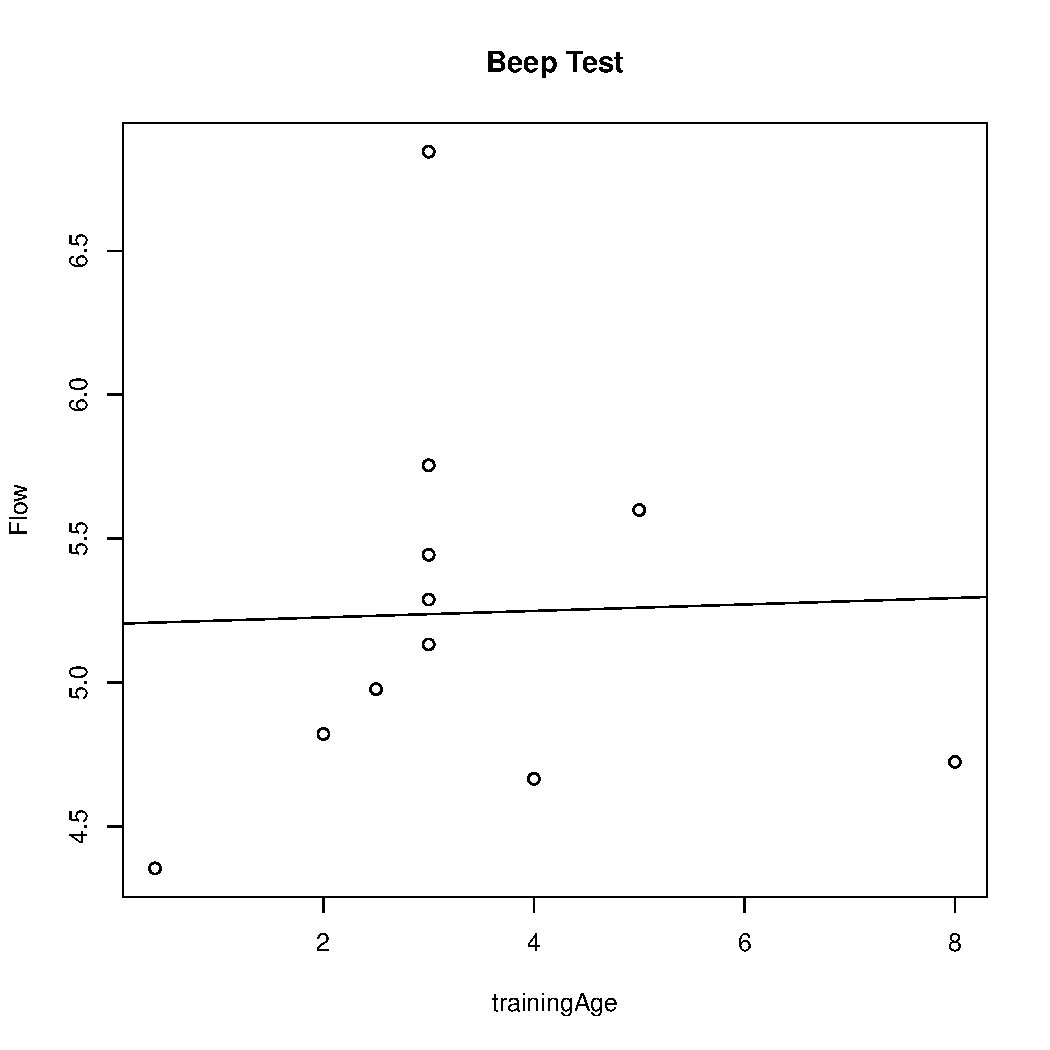
\includegraphics[scale=.2]{images/beepFlowTrainingAge.pdf}
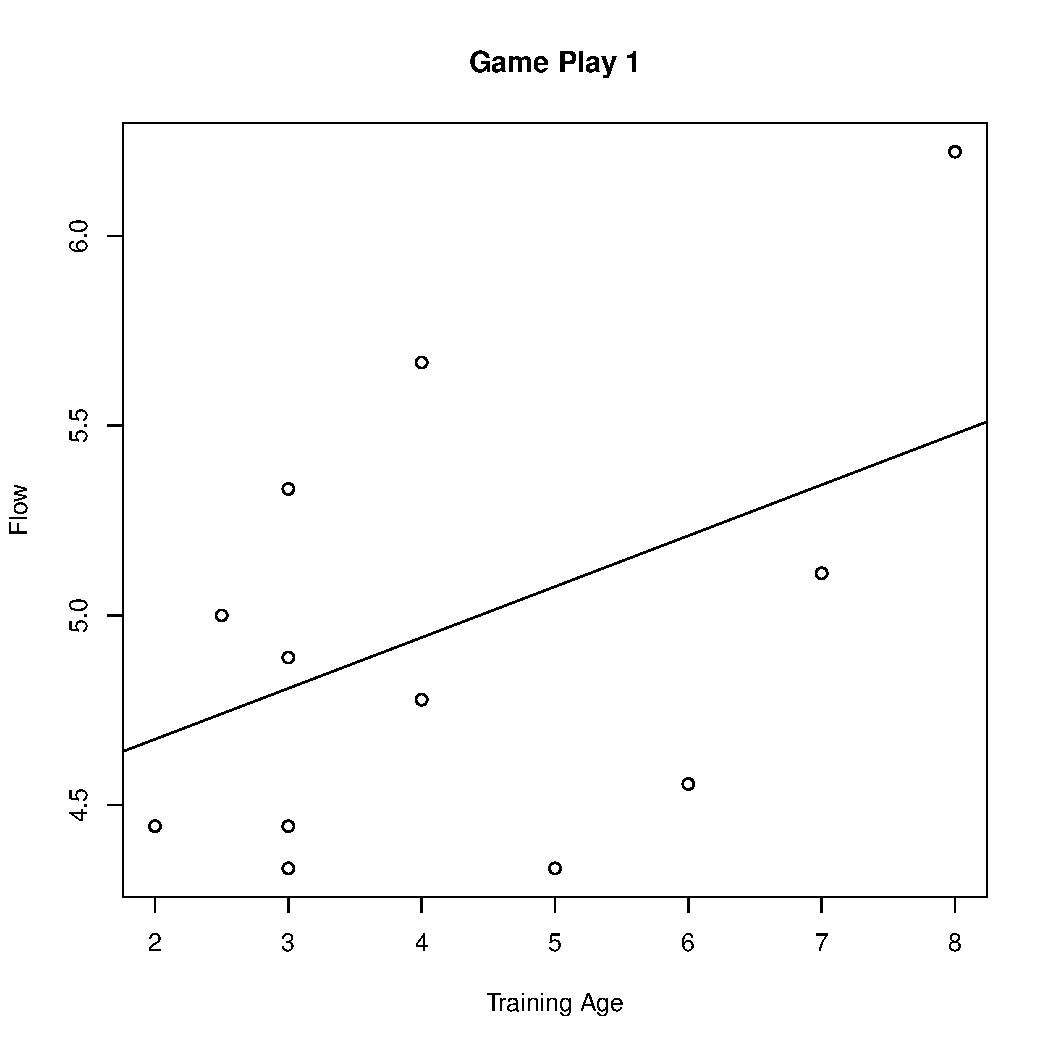
\includegraphics[scale=.2]{images/flow0109TrainingAge.pdf}
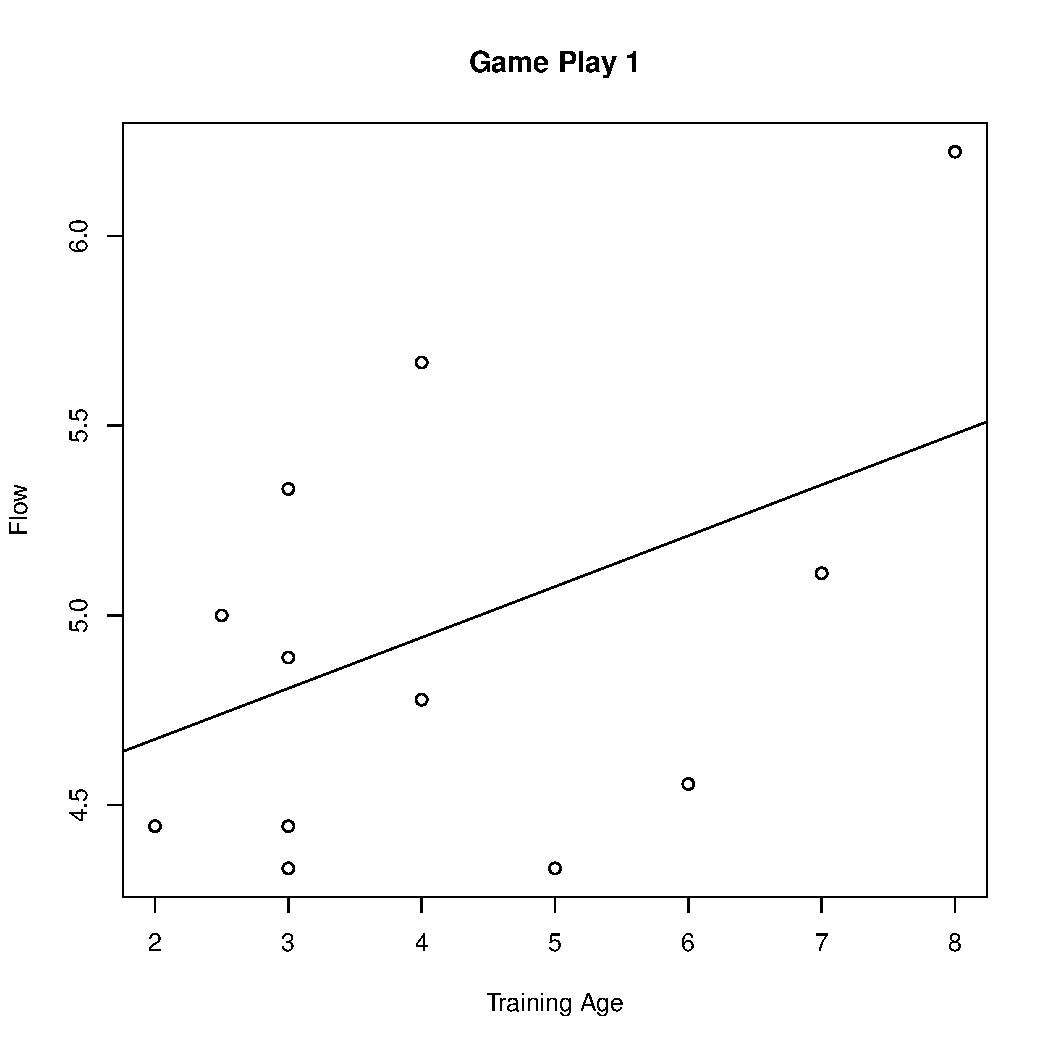
\includegraphics[scale=.2]{images/flow0109TrainingAge.pdf}
  \caption{Flow State by Training Age in three training sessions (Beep Test, Match Sim 1, Match Sim 2)}
  \label{fig:flowTrainingAge}
\end{figure}

Analysis of responses to individual items of the Flow state scale ( ``Just now I did not care how others would evaluate me'' (Evaluation From Others) and  ``Just now I did not care how I performed'' (Self Performance)) revealed variation according to training session type.   In a comparison between the Beep Test and Game Play 1, the mean value for Evaluation From Others was higher in the Beep Test ($M = 5.25 SD = 1.35$) than in the Game Play 1 ($M = 3.15 SD = 1.95$) session, ($two-sample t(19.94) = 2.77, p = 0.01$).   The mean value for Self Performance was also higher in the Beep Test ($M = 4.32 SD = 1.74$) than in the Game Play 1 ($M = 1.92 SD = 1.32$) session, ($two-sample t(15.06) = 6.06, p < 0.001$).

In a comparison between the Beep Test and Game Play 2, the mean value for Evaluation From Others was higher in the Beep Test ($M = 5.25 SD = 1.35$) than in the Game Play 2 ($M = 3.67 SD = 2.19$) session, ($two-sample t(21.84) = 2.00, p = .05$).   The mean value for Self Performance was also higher in the Beep Test ($M = 4.32 SD = 1.74$) than in the Game Play 2 ($M = 2.93 SD = 2.22$) session, ($two-sample t(15.06) = 6.06, p < .001$).  Mean scores of these two items appeared to differ according to junior and senior athlete for both Game Play sessions, but no differences were significant (all $p’s > .29$).

Scatter plots (see Figures ~\ref{fig:othersEvalPostTraining} and ~\ref{fig:indPerfPostTraining}) reveal a general trend in which more positive answers to these two items appear to correlate with higher training age, such that more experienced athletes appear to be less concerned about their own performance and the evaluation by others.  Correlations between these variables were not significant (all $p’s > .09$).

\myparagraph{Discussion}
This survey study was conducted opportunistically and without necessary randomisation or control required for causal inference.  Results do, however, offer some reinforcement of ethnographic evidence. First, results revealed a difference in experience of flow between the Beep Test and the Game Play sessions, suggesting that the level of uncertainty in joint action could be one possible factor (among others) contributing to this observed difference. Further investigation of this possibility would require a controlled experimental design in which uncertainty in joint action was systematically varied or controlled (see ~\ref{chap:trainingExperiment}).  Second, results suggest a possible association between athlete training age and and reports of Flow, such that athletes more experienced with rugby’s joint action demands on average experienced higher levels of flow  in the Game Play sessions than athletes less experienced with joint action in rugby.








\subsubsection{Athletes experience positive violations of expectations concerning performance\label{sect:expectationViolation}}
The data presented thus far emphasises on-field performance as a source of psychological stress for athletes. At the same time, I also documented evidence that athletes derived considerable joy and motivation from successful performance.  The vignette in which I describe Hongwei's journey from timid novice to exhilarated junior team member serves as an emblematic example of this phenomenon (See Chapter ~\ref{chap:theory} Section ~\ref{sect:SHW}).  In this section, I present more evidence that bears upon Hypothesis 2, i.e., that more positive violations concerning team performance will generate higher levels of team click and, in turn, higher levels of social bonding.

In addition to Hongwei, I noticed many other athletes gradually develop---and at times impressively deploy---a ``feel for the game'' on the training field and in competition.  My discussions with athletes in interviews confirmed the fact that athletes derived considerable motivation from the experience of discovering that they were suddenly capable of performing one aspect of rugby's diverse technical skill set.  Athletes recount with unmistakable energy and elation the moment in which their previously held expectations around individual and team performance were \textit{positively} violated.

Wang Zhengfeng offered one powerful example of athlete experience of positive violation of expectations around performance in rugby.  Wang Zhengfeng was a very talented, but still inexperienced, athlete, who had converted from athletics to rugby in 2012.  He was an athlete with outstanding physical attributes for rugby---particularly speed, agility, and strength.  Wang struggled, however, to master some of the basics of rugby's game play, such as catching, passing, and tackling. I asked Wang about his approach to the challenge of learning the skills of rugby from scratch, and he recounted the time he first discovered that he could execute a ``side step'' (a technique used by the ball carrier to evade oncoming defence):

    \begin{quote}
      JT: How do you overcome this challenge [of learning new skills in rugby]? Do you have a specific plan or way of approaching it? \\
      WZF: I imitate.  Like when I was learning how to sidestep. At the time I’d look at Brother Han (Han Xiaolong) who has a really good sidestep. I'd just watch him stepping.  Every day I'd just watch him step, and imitate him.  At the start I probably wasn't practicing it particularly well, I couldn't quite imitate it, but then after some time, I was playing touch and suddenly produced the exact action! I was so happy! Its not like it appeared at a fixed time or anything, it was like suddenly I just moved a step and it happened. And then like after I stepped once I slowly found the feeling, and then stepping became my own thing.  When you pick up new skills for the first time it feels very addictive, I get so happy, when it happens I can stay happy for a long time!
    \end{quote}

    \begin{quote}
      JT: 那你自己通过什么样的方式克服这个困难,你有计划和想法吗? \\
      WZF:模仿。就像变相一样,我当时看龙哥做的特别好,我就看他们变向,天天就看哎,模仿一下,可能开始练得不是特别好,模仿不大会,但是时间长了以后,打TOUCH的时候突然做出了这么一个动作!就特开心! 对没有固定的时间出来的,突然动了一步就出来的。比如变向突然出来之后,慢慢就找到感觉了,变相就变成自己的东西了. 做出来新的动作以后就觉得很过瘾,特别开心,能开心很长时间了!
    \end{quote}

Wang was an athlete who experienced a lot of performance-related anxiety.  Given his physical attributes and his obvious potential to be an effective rugby player (he was, for example, one of the fastest professional rugby players in China), he and the people around him (coaches and other senior athletes) held high expectations for his performance.  Often Wang felt like he didn't live up to these expectations.  When Wang did experience the feeling of perceived success in joint action, however, he felt elation that could last for ``a long time'' afterwards.  Importantly, Wang's description above indicates that the surprise of the phenomenon is an important dimension to its emotional valence.

The young hopeful athlete Yang Can, a junior athlete who also had impressive physical attributes for rugby, but was incredibly timid, gave a more low key response to a similar discussion in our interview:

    \begin{quote}
      When I first started practicing, ok, I’ll just carry the ball forward and hit it up [that was all I could do]. After that, I discovered that there are many techniques: you can fend people, you can step, you can run into a gap. There are many other actions (than just running straight towards the defence with the ball).
    \end{quote}

    \begin{quote}
      刚开始练得时候就是拿着球往前跑,撞呗,后来发现有好多技巧,也可以推人,也可以变向,也可以走空档,有很多其他动作
    \end{quote}

While the words on the page perhaps don't quite jump out in the same way that Wang's description does, Yang Can's description of his discovery of rugby's many techniques was a bright and animated spark in an otherwise reserved interview, in which many of his responses rarely involved more than a few sentences (and often only a few word per sentence!).  His joy in describing the sensation of discovering new dimensions to his technical repertoire was clear.

These two examples relate more closely to the category of individual performance.  I also found evidence that positive expectation violation applied to team performance.  As senior player Han explained, he only began to really enjoy rugby when he had an opportunity to coordinate with others:

\begin{quote}
    When I first started training for rugby, when I first started getting exposed to contact I was a little bit afraid, but then after I have been exposed for a longer time I became less and less afraid of contact, and then I felt more and more that as I added a few more things...like when I started to find that coordination between players when playing touch...Because I really enjoy that sort of ``two people coordinating---``pa-pa-pa'' [describing the action of coordinating movement and passes on the field in rugby] passing between players and breaking through the line'' type of feeling, I really enjoy it.
\end{quote}

\begin{quote}
      刚开始练橄榄球的时候,刚接触对抗的时候有点害怕,但是接触的时间长了以后就越来越不怕对抗,后来越来越觉得就加了一些,会打的打TOUCH的时候相互之间有配合,因为我特别享受那种两个人配合怕怕怕配合传球最后突破的这种感觉我特别享受.
\end{quote}

In a similar vein as both Wang and Yang, Han's animated description of the feeling of ``two people coordinating (pa-pa-pa)'' elicits a positive emotional valence surrounding moments in which expectations around performance are either met or exceeded.  In addition to his description of discovering his ability to side-step, Wang Zhengfeng also offered an animated description of the phenomenon of tacit understanding in joint action:

  \begin{quote}
    It’s really hard for me to say what it feels like.  It feels just like a fight for life or death, like you must win the match.  Normally, that sort of tacit understanding sometimes isn’t there, but then suddenly you coordinate on the field and you can form this feeling.  You haven't given much consideration as to how to play...its probably also to do with the feeling of time spent together, the few of us know each other’s characteristics, we understand each other relatively well.  Its like sidestepping, suddenly you can get that feeling of tacit understanding.
  \end{quote}

  \begin{quote}
    还真说不出来是什么感觉。就是感觉生死战一样,必须要拿下来他。那种默契平时有的时候没有,在现场上突然配合就感觉打上来了这种感觉。没有考虑太多怎么打,可能也是时间长的感觉,我们几个知道自己的特点,彼此可能比较了解,跟变相一样,突然就出来了那种默契的感觉
  \end{quote}

Wang had just described to me his exhilarating discovery of the side-step, and so the use of the side-step to articulate an analogous phenomenon on the team level was convenient.  Nonetheless, it serves to capture the surprising and sudden sensation of successful performance in joint action.


SUMMARISE EXPECTATION VIOLATION:
* Examples occur as part of a transition from novice to skilled?
    * could be a link with development of technical competence
    * Support for H21, H22, H23, but what about H24?


















\section{Discussion}


















                                                          \end{CJK}
